% !TEX root = ../../../main.tex
% 来源：中学数学实验教材·第三册（高中数学）
% 章节：函数及其图象 / 一次函数（线性函数）
% 原始文件：4.tex，行 2202-2220
% 类型：tikz
% ---
    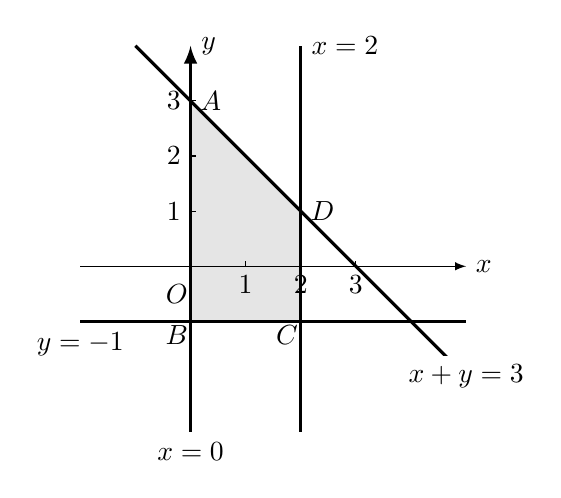
\begin{tikzpicture}[>=latex, scale=.7]
        \fill [gray!20](0,-1)--(2,-1)--(2,1)node[right, black]{$D$}--(0,3)node[right, black]{$A$}--(0,-1);
    
    
        \draw[->] (-2,0)--(5,0)node[right]{$x$};
        \draw[->,very thick] (0,-3)node[below]{$x=0$}--(0,4)node[right]{$y$};
        \node at (-.25,-.5){$O$};   
        \foreach \x in {1,2,3}
        {
            \draw (\x,0)node[below]{$\x$}--(\x,.1);
            \draw (0,\x)node[left]{$\x$}--(.1,\x);
        }
        \draw [domain=-1:5, samples=10, very thick] plot(\x, {3-\x});
        \draw[very thick] (-2,-1)node[below]{$y=-1$}--(5,-1);
        \draw[very thick] (2,-3)--(2,4)node[right]{$x=2$};
    \node at (5,-2) [fill=white]{$x+y=3$};
    \node at (0-.25,-1-.25){$B$};
    \node at (2-.25,-1-.25){$C$};
    \end{tikzpicture}
